%--------------------------------------------------------------------------
%
%                                                    SOLUTION
%
%--------------------------------------------------------------------------

\begin{center}
\vspace*{5mm}
\noindent {\Large {\bf (Solution) }}
\end{center}


\begin{enumerate}
\item[a) ] 
We start from the equation of motion
\[
\ddot{x}(t) =  a,
\] 
which is integrated once to find the speed as a function of time.
\begin{equation}
\dot{x}(t) = at + cte.
\label{eq_premiereintegrale}
\end{equation}
To find the integration constant, expression (\ref{eq_premiereintegrale}) is evaluated at instant $t=0$: 
\[
\dot{x}(t=0) = 0 + cte. 
\]
Therefore, the integration constant is equal to the speed evaluated at instant $t=0$. This initial speed is noted $v_0$. We integrate once more to find the position as a function of time

\begin{equation}
x(t) = \frac{1}{2}at^2 + v_0 t + cte'.
\label{eq_deuxiemeintegrale}
\end{equation}

Again, this expression is evaluated in $t=0$ to find the integration constant.
\[
x(t=0) = 0 + 0 + cte'.
\]

The integration constant is equal to the position evaluated at time $t=0$. That's the initial position, denoted $x_0$. Finally, we find that the solution of the equation of motion $\ddot{x}(t) =  a$ is, indeed, $x(t) = \frac{1}{2}at^2 + v_0 t + x_0$ where $v_0$ and $x_0$ represent, respectively, the initial speed and position.
We can check that by deriving $x(t)=\frac{1}{2}at^2+v_0t+x_0$ twice with respect to $t$, which yields:

\[
\ddot{x}(t) \equiv \frac{d^2x(t)}{dt^2} = \frac{d^2}{dt^2}\left(\frac{1}{2}at^2+v_0t+x_0\right)
\]
\[
= \frac{d}{dt}\left(\frac{1}{2}a2t+v_0\right) = \frac{d}{dt}\left(at+v_0\right) = a.  
\]
This verifies the equation of uniformly accelerated rectilinear motion.


\item[b) ] \textbf{Understanding the problem:} the most efficient way of understanding and interpreting the problem is to draw a \emph{big} representation of all the data available (as shown below). The considered system is the salmon, with its origin at the lake's surface. At $t=0$, the salmon jumps out of the lake at position $x_0=0$ and with vertical upwards initial speed $v_0$. Throughout the jump, gravity subjects it to a constant acceleration $-g$. Its position as a function of time is given by equation (\ref{eq_deuxiemeintegrale}), and its speed as a function of time by equation (\ref{eq_premiereintegrale}), in which we set $a=-g$.

\begin{center}
{\input{figures/serie01_c_fig1.pdf_t}}\\
\end{center}
\hspace*{15mm}
\begin{figure}
\begin{center}
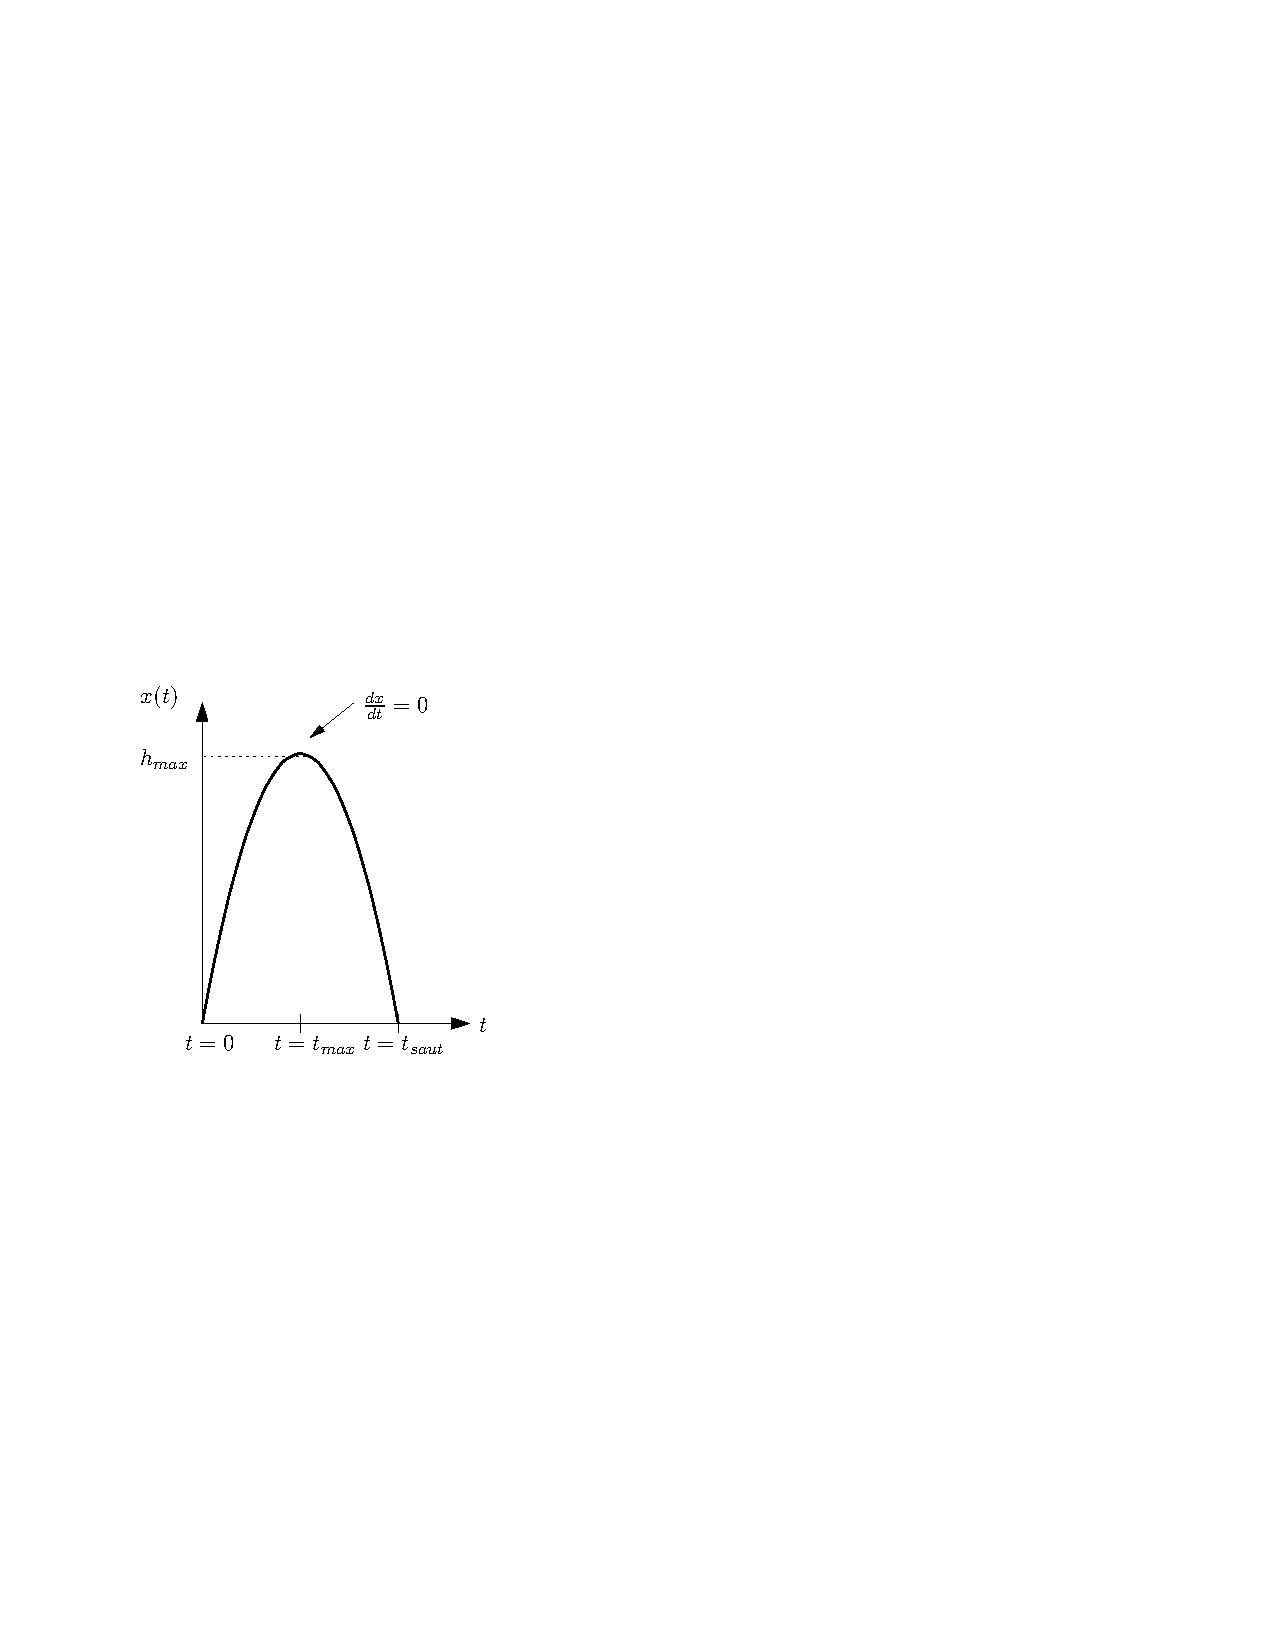
\includegraphics[width=.45\textwidth]{figures/serie01_c_fig1-2b.pdf}
\vspace{.05\textwidth}
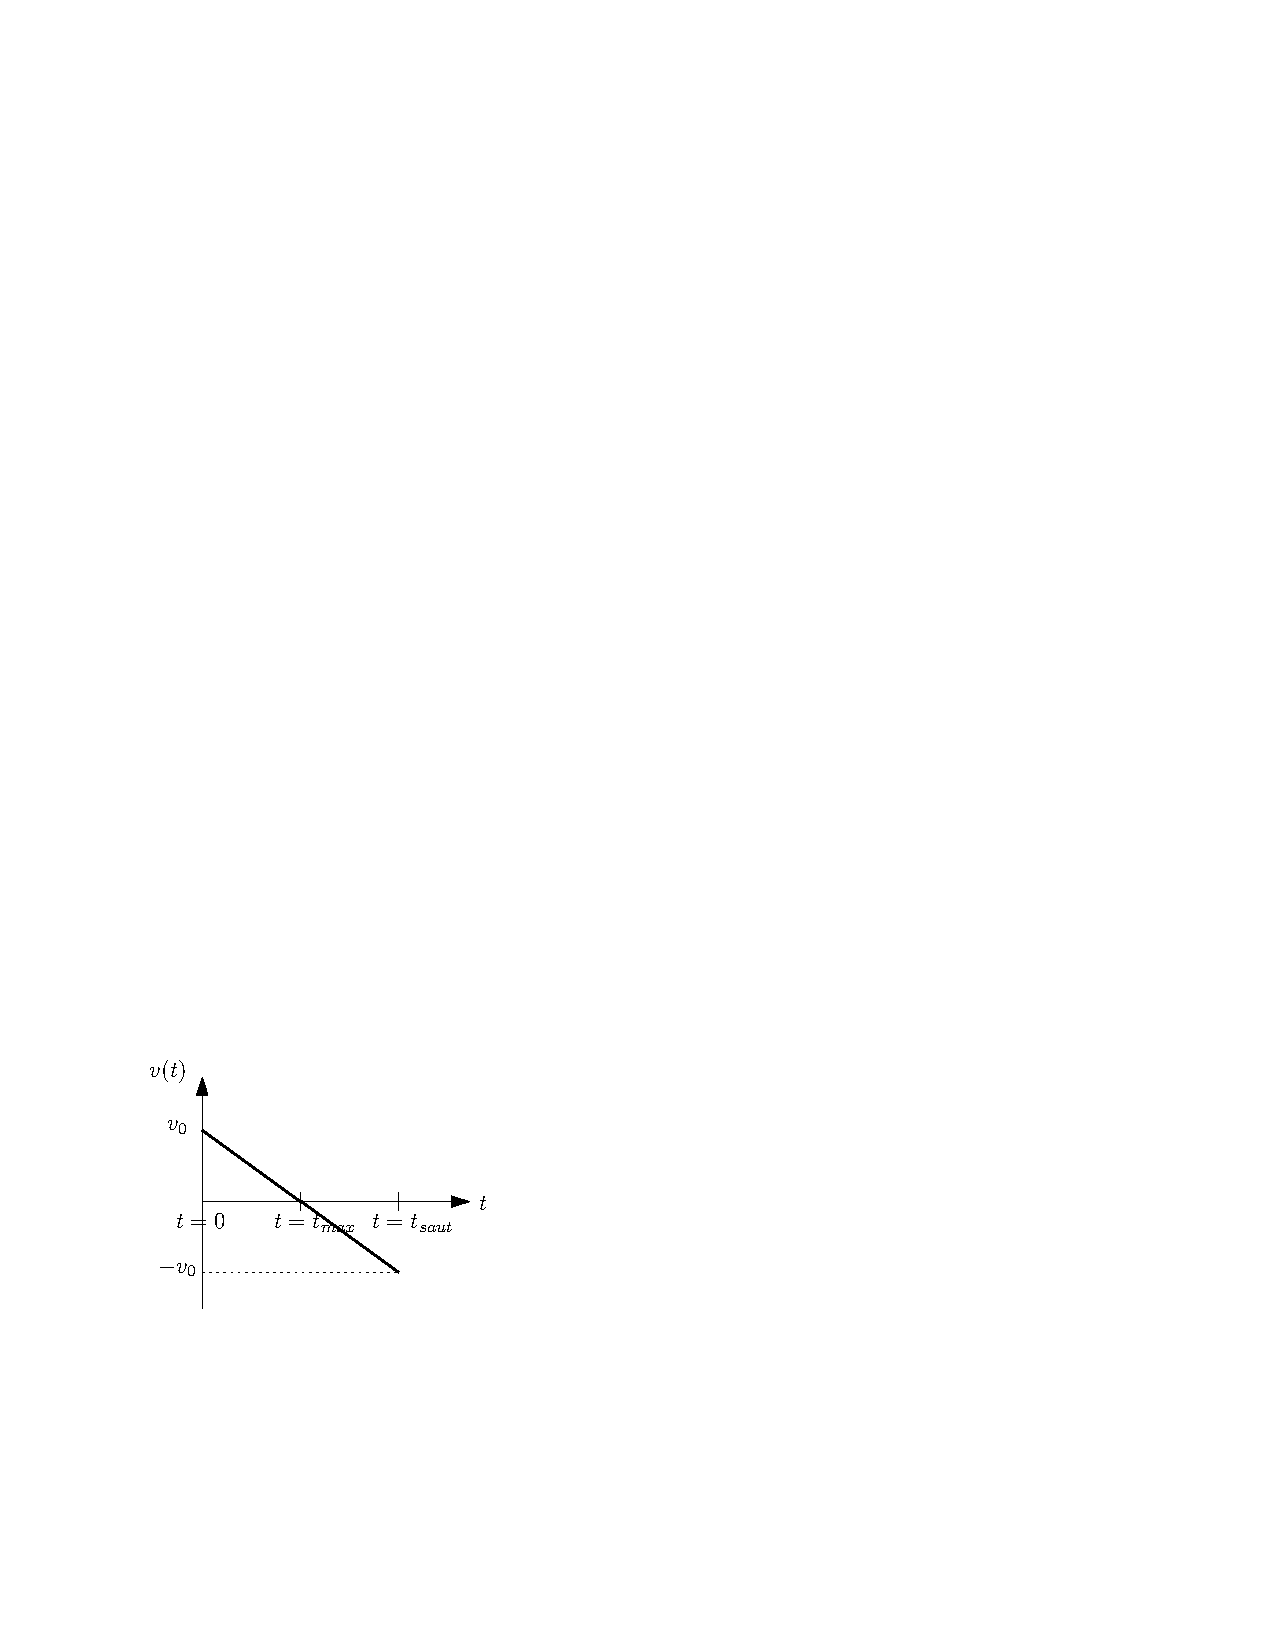
\includegraphics[width=.45\textwidth]{figures/serie01_c_fig1-2c.pdf}
\end{center}
\end{figure}
\vspace{0.9cm}


Graphically, the position and the speed as a function of time are given in the two figures above. Noticeably, 
\begin{itemize}

\item The position as a function of time is a second order polynomial. Graphically, that's a parabola.
\item The parabola's peak is the maximal height reached by the salmon, at an instant we shall label $t=t_{\rm max}$.
\item The salmon's speed decreases linearly. Graphically, that's represented by a straight line. The slope of that line is the salmon's acceleration.
\item At $t_{\rm max}$, the line crosses the $t$-axis: the salmon's speed is naught at the top of its trajectory. At any given time, the speed corresponds to the derivative of the position with respect to time. At time $t_{\rm max}$, null speed corresponds to the peak of the parabola, which is indeed of null slope.
\item The parabola is symmetrical. Let $t_{\rm jump}$ be the time at which the salmon falls back into the water. Then $x(t_{\rm jump}) = 0$ et $t_{\rm max}= \frac{1}{2}t_{\rm jump}$.  
\end{itemize}
\item[c) ] 
\begin{itemize}
\item \textbf{Solving process(es):} We're trying to find the maximal height reached by the salmon and the time it spends in the air. To do so, the steps to follow are:

\begin{itemize}
\item[-] Integrate once the equation of motion $\ddot{x}(t)=a$ to find the speed as a function of time, then integrate again to find the position as a function of time.
\item[-] Use the limiting conditions to solve these equations. \\
\end{itemize}
 \item \textbf{Choice of process and resolution:} 
The first part of the process has been carried out in part a). We use equations
 (\ref{eq_premiereintegrale}) and (\ref{eq_deuxiemeintegrale}) for which $a=-g$ et $x_0=0$:
\[
x(t) = -\frac{1}{2}gt^2 + v_0 t \quad \textrm{et} \quad v(t) = -gt + v_0. 
\]
At the top of the trajectory (final condition), the salmon reaches a height $x(t_{\rm max}) = h_{\rm max}$ at time $t_{\rm max}$. At that instant, its speed is naught: $v(t_{\rm max})=0$. 
\[
-gt_{\rm max} + v_0=0 \Rightarrow t_{\rm max} = \frac{v_0}{g}.
\]
Plugging that result in the equation that describes the position as a function of time yields

\[
h_{\rm max} = -\frac{1}{2}gt_{\rm max}^2 +v_0 t_{\rm max} = -\frac{1}{2}g\frac{v^2_0}{g^2} +v_0 \frac{v_0}{g} = \frac{1}{2}\frac{v_0^2}{g}.
\]
Finally, we compute $t_{\rm jump}$, the overall time the salmon spends in the air, by using the final condition $x(t_{\rm jump}) = 0$:
\[
-\frac{1}{2}gt_{\rm saut}^2 + v_0t_{\rm saut}=0 \Rightarrow t_{\rm saut}=0 \mathrm{(solution\; \grave{a}\;\acute{e}viter)\;ou}\;t_{\rm saut} = \frac{2v_0}{g}.
\]
This result confirms that $t_{\rm max} = \frac{1}{2}t_{\rm saut}$, as expected.

\emph{Numerical application:} \\$v_0=3\,\mathrm{m/s}$ et $g=10 \,\mathrm{m/s^{2}}$ donc $t_{\rm jump} = \frac{2v_0}{g} = \frac{2\times 3}{10}=0.6\,{\rm s}$ et $h_{\rm max} = \frac{1}{2}\frac{v_0^2}{g} = \frac{3^2}{2\times10}=0.45\,{\rm m}$. \\

\item \textbf{Discussing the results:} The results we found\ldots\\
\begin{itemize}
\item[-] \ldots are in the right units: for $t_{\rm jump}$, we expect a result in seconds. $\frac{2v_0}{g} \rightarrow \frac{m/s}{m/s^2} = \frac{m}{s}\frac{s^2}{m} = s$. \\
For $h_{\rm max}$, we expect meters: $\frac{1}{2}\frac{v_0^2}{g} \rightarrow \frac{(m/s)^2}{m/s^2} = \frac{m^2}{s^2}\frac{s^2}{m} = m$. \\
\item[-] \ldots are in the right order of magnitude: $v_0 \simeq 10^0$ m/s and $g \simeq 10^1$ m/s$^2$. Therefore, $t_{\rm jump} = \frac{2v_0}{g} \simeq \frac{10^0}{10^1} \simeq 10^{-1}$ s and $h_{\rm max} = \frac{1}{2}\frac{v_0^2}{g} \simeq \frac{10^0}{10^1} \simeq 10^{-1}$ m. It seems reasonable that the salmon would jump a few tens of centimetres, and that the jump would last a few tenths of seconds. \\
\item[-] \ldots has the correct signs: $h_{\rm max}$ must be positive, since it is on the positive side of the vertical axis (see figure). Indeed, $\frac{1}{2}\frac{v_0^2}{g} > 0$. $t_{\rm jump}$ must also be positive, since the salmon falls back into the water after having jumped, and not before. Indeed, $\frac{2v_0}{g}$ > 0. \\
\item[-] \ldots is coherent with limiting cases. If $v_0 \to \infty$ (the salmon jumps at very high speed), then  $h_{\rm max} \to \infty$ (it reaches a very high point) and  $t_{\rm jump}\to \infty$ (the jump lasts a very long time). We can make a similar case for $v_0 \to 0$. \\
\end{itemize}
\end{itemize}

\end{enumerate}
